\chapter{Conclusion}
\label{sec:conclusion}

\dictum{… except in the light of genetics.\par\dictumrule}

\noindent
Evolution by natural selection is the implicit assumption underlying all of
modern biology. \citet{Dobzhansky:1973} famously argues against ill-informed
criticism of evolution, stating that

\begin{quote}
    Nothing in biology makes sense except in the light of evolution.
\end{quote}

This statement is as relevant today as it was then --- both as an admonishment
about the still prevalent ignorance of basic biological facts, and serving as a
succinct summary of our understanding of biology. In fact, modern evolutionary
synthesis, which is the prevailing explanatory model employed today, and which
is itself an evolution of the Darwinian theory of descent with modification by
means of natural selection, is unchallenged in this status, and is corroborated
by every new piece of evidence.

In \texttitle{The making of the fittest}, Sean Carroll argues that the best
evidence for evolution we have is the genetic record that we can now read
directly in the \dna of all living species \citep{Carroll:2006}. Carroll was
mainly talking about the similarity between homologous genes in different
species. But one of the most striking examples of strong conservation is the
near-universal genetic code: Throughout billions of years of evolution, the
instruction set used to encode the building blocks of proteins has remained
virtually unchanged.

In contrast with the conservation of the genetic code itself, the implementation
of this code shows some degree of variation, most notably in the variation of
the selection of preferential synonymous codons (reviewed in
\citet{Ermolaeva:2001}) on the one hand, and in the divergence of the \trna
genes \citep{Kutter:2011} on the other hand.

\section{Discussion}

\subsection{Regulation of \abbr{trna} gene expression}

In \cref{sec:trna}, I have summarised our research into the variability of the
\trna genes, not across evolution, but across development. Our findings mirror a
common theme: despite pervasive variation of \trna gene expression, the
anticodon isoacceptor \trna abundance remains very stable across different
stages of development, and matches the codon demand of the transcriptome which,
itself, also shows very little variation.

As there is no effect on the abundance of the \trna anticodon isoacceptor pools,
it remains unclear why such variation of the \trna gene expression exists;
however, I have shown that the variation is not stochastic but rather the
product of coordinated regulation, precisely to ensure the stability of the
anticodon pool. One might thus suspect that the observed variation in \trna gene
expression is simply a consequence of a stabilising mechanism to provide a
buffer against extrinsically caused changes in the expression of individual
\trna genes.

On the other hand, the variability in \trna gene expression may be due to a
regulatory role, which is a common theme of \ncrna[s]: Many different types of
\ncrna are known to be implicated in the regulation of gene expression through a
variety of mechanisms \citep{Mattick:2006}. For example, \lncrna[s] have been
shown to bind to chromatin and help shape its conformation \citep{Rinn:2012},
and small \rna fragments from different sources are involved in \rna silencing
via a machinery known as \risc \citep{Hamilton:1999,Hammond:2000}.

Although \trna[s] have a “canonical” role — to act as adapters in the process of
translation — this of course does not preclude other roles. In fact, there is
evidence that ties \trna-derived fragments to different regulatory roles. As
mentioned in the introduction, about ten per cent of the bases in the \trna[s]
transcript are post-transcriptionally modified. Some of these modifications
impact the stability of the transcript. For example, it is known that
cytosine-\num{5} methylation in the anticodon loop of \trna[s], which is
prevalent in actively transcribed \trna[s], inhibits endonucleolytic cleavage.
Absence of this methylation leads to cleavage and the accumulation of \threep
and \fivep fragments \citep{Thompson:2008}. Furthermore, there is evidence that
overabundance of \fivep \trna fragments lead to cellular stress
\citep{Blanco:2014}.

But not only the \fivep fragment of \trna[s] is catalytically active: the
\threep ends of specific \trna[s] have been shown to act as primers for the
transcription of endogenous retroviruses such as \hivi \citep{Litvak:1994} in a
highly sequence-specific manner. In general, the expression of such retroviruses
is detrimental for the cell and, by implication, excess abundance of specific
\trna-derived fragments affects the cell’s fitness negatively. This exerts a
selective pressure to evolve a mechanism for suppressing such fragments. One way
of depleting their abundance is to downregulate the expression of originator\todo{ugly, better word?}
\trna genes in response to the detection of excess \trna fragments.

In sum, the regulatory role of \trna transcripts adds another dimension to the
need for the regulation of their abundance. In fact, the dependence on specific
enzymes (such as \protein{mmu}{NSUN2} in mouse) to methylate \trna[s], and thus
to ensure their stability hints at the fundamental importance of preventing the
formation of excess \trna-derived fragments \citep{Blanco:2014}.

The precise mechanism of the \trna gene expression regulation remains unclear.
Corroborating previous reports \citep{Oler:2010}, I have found some evidence
that \trna gene activity correlates with specific histone marks. However, it is
unclear whether this is a cause or a consequence of differential regulation, and
it is insufficient to account for differences in the expression of \trna genes
in close vicinity. Furthermore, there is so far no mechanism for the dynamic
feedback necessary for effecting the compensatory effect between genes in an
isoacceptor family.

\subsection{Absence of evidence for codon bias-dependent translation efficiency in mammals}

Despite the existence of larger variations in codon usage between subsets of
genes, some of which are cell type specific, I was unable to find evidence for a
regulatory effect of this codon bias on translation rates via higher adaptation
to a cell type specific \trna anticodon isoacceptor pool in mammals. On the
contrary, the variation in the \trna anticodon abundance does not seem to
correlate with cell type specific codon demand. This finding, presented in
\cref{sec:codons} lends support to a view that has recently been challenged
\citep{Gingold:2014,Wilusz:2015}: that translational selection via codon bias,
if present at all, plays a negligible role in mammalian systems. It will be
interesting to see how this controversy will unfold.

If true, this implies that codon bias has not conserved the regulatory role it
plays in unicellular organisms of all domains of life \colorbox{yellow}{REF},
where it is well established that codon bias influences translation efficiency
to control gene-specific expression levels. Why would this central role of codon
bias be present in unicellular organisms but not in complex multicellular
animals? The following is an attempt at an explanation.

In contrast to unicellular organisms, multicellular organisms need to encode the
fundamentally different functionality of distinct cell types in a single, static
genome. This is achieved through a highly sophisticated regulatory machinery
whose dynamic evolution has been revealed in recent years, in particular with a
focus on mammalian systems \colorbox{yellow}{REF, Berthelot}. While  organisms
consisting of a single cell type also employ gene regulatory networks, the
complexity of the regulatory machinery in organisms with many cell types is much
higher in comparison, and in particular relies heavily on distal regulatory
elements and epigenetic modification.

However, despite only consisting of a single cell type, unicellular life still
needs to dynamically adapt to different environments. Besides using simple
transcriptional control, they also rely heavily on translational control by
means of gene specific codon bias variation. In multicellular organisms, the
existence of a more direct control of gene expression via transcription
regulation obviates the need for this less direct mechanism.

The effect this has is further heightened by the simpler genomic \trna landscape
in unicellular organisms: while mammals have several hundred \trna genes, with
up to dozens of gene copies per anticodon, unicellular organisms possess fewer
anticodons, and usually just a single \trna gene copy per anticodon
\citep{Chan:2009}. As a consequence, the downregulation of even just a single
\trna gene copy has profound consequences on the cytosolic \trna concentration,
and thus the ability of the cell to translate individual codons. This acts as a
powerful pressure on the selection of suitable codons.

I suggest that these two factors — the relatively higher complexity of
transcriptional regulation in mammals, and the higher impact of variation in
\trna gene transcription on variation in
\trna availability and thus on translation efficiency in unicellular organisms —
is sufficient to explain the results we observe here as well as established
results reported in the literature.

At the end of the project outlined in \cref{sec:codons}, I have started
exploring other potential sources of the cell type-specific codon bias observed
in mammals, unrelated to the regulation of translation rate. My first intuition
was that the codon bias might be a stochastic artefact caused by the small size
of the gene sets under consideration. However, whilst stochastic variation does
have an effect on codon bias, it is insufficient to explain all the observed
codon bias in most gene sets. I will continue exploring genomic \gc bias as
another potential cause of this effect.

\subsection{The extended \abbr{pol3} transcriptome}

The \pol3 \chipseq data generated for the projects presented in this thesis
provides a wealth of information beyond just \trna gene activity.
\Cref{sec:pol3} takes a brief glimpse at genome-wide \pol3 binding and confirms
that \pol3 binding can be used to assess gene activity of genes with known
\pol3-driven transcription.

In particular, I was able to assess binding of \pol3 to the promoter region of
\transsine loci. The problem of multi-mapping reads and the high number of
\transsine gene copies makes it hard to assess the activity of individual
\transsine genes. However, by collapsing \transsine gene families, I could
corroborate previous reports of \transsine transcription in vivo
\citep{Carriere:2012}.

\section{Future directions}

\subsection{Regulation of \abbr{trna} transcription}

While providing unprecedented insight into the controlled variability of \trna
gene transcription, \cref{sec:trna} has failed to establish a mechanism for the
differential regulation of \trna gene transcription. Known features of \pol3
recruitment, such as transcription factor binding and specific histone marks,
could not conclusively be shown to cause the differences I observed in the \trna
gene transcription between different stages of development. My analysis
deliberately excluded the internal promoters of \trna genes from the search for
specific motifs since it has previously been reported that variation of the
internal promoter of \trna genes is unrelated to variation in gene expression
\citep{Oler:2010,Canella:2012}.

However, results in \citet{Gingold:2014} indicate that this may have been
premature, as they find significant differences in the B box of \trna genes
which they reported as differentially expressed between conditions. This
suggests that internal promoter variation may contribute to the observed
variability of the \trna transcriptome after all. I intend to run the methods
they used on our data to test this hypothesis.

\subsection{Codon usage adaptation}

The question of what causes codon usage bias variability across functional
subsets of the transcriptome remains wide open. \gc bias, in particular, is
worth exploring further. On the one hand, I observed a robust correlation
between \gc bias and codon usage, and we know that codon usage can sometimes be
predicted from intergenic \gc bias \citep{Chen:2004}. On the other hand,
\citet{Duret:2002} show that, at least in \species{dmel} and \species{cel}, \gc
bias is uncorrelated with codon usage bias.

To explore this further, two avenues present themselves:

\begin{enumerate}
    \item It is known that intergenic isochore \gc content in mammals predicts
        codon usage. Since intergenic regions are non-coding, this suggests that
        differential codon usage between genes has, at best, a minor functional
        relevance. So far, I have only looked at \gc bias in coding sequences.
        To make similar conclusions, I will have to instead compare codon usage
        to the \gc bias in the flanking regions of protein-coding genes.
    \item \gc bias can vary between synonymous and non-synonymous codons. If \gc
        bias is indeed causal for codon usage, we would expect that \gc bias
        correlates highly between the first two nucleotide positions of the
        codon and its wobble position. However, if the wobble position’s \gc
        bias is uncorrelated to the \gc bias of the other codon positions in a
        gene set, this would require a different explanation.
\end{enumerate}

Another feature known to constrain codon deployment is the presence of other
sequence features in the coding region of genes. This includes binding sites for
enhancers and splicing factors \citep{Hyder:1995,Blencowe:2000}. The extent of
this constraint has recently been shown to be much more widespread than
previously assumed \citep{Stergachis:2013}. It is conceivable that condition
specific gene sets carry enhancers for their own transcription in their gene
bodies, which would contribute to a codon usage bias. It would be worthwhile to
investigate the enrichment of such binding sites in gene sets with strong codon
bias, in particular those reported by \citep{Gingold:2014}.

The usage of a simple correlation between matching codons and anticodons,
disregarding wobble base pairing, has proved adequate to demonstrate an overall
high correlation between the codon demand and matching \trna anticodon
isoacceptor pool. However, arguing about the relative adaptiveness of different
gene sets or transcriptomes may make it  necessary to consider wobble base
pairing to model the codon--anticodon interaction more precisely. The \tai
\citep{Dos_Reis:2003} offers a way of quantifying codon--anticodon adaptation by
considering (simplified, see \cref{tab:wobble}) wobble base pairing rules.
However, it is conventionally based on the \trna isoacceptor gene copy number as
a measure of anticodon abundance. I plan to improve this using our \trna gene
expression data, which offer a more accurate anticodon isoacceptor abundance
measure, instead. In addition, it may be possible to extend the \tai metric by
considering extended wobble base pairing rules \citep{Murphy:2004} --- although
it is likely that this will have a very limited effect on the adaptation value.

\subsection{\abbr{Pol3} transcription of \abbr{transsine}s}

The next step in the analysis of \transsine expression requires a framework for
the robust quantification of \pol3 binding signal over background noise. I
intend to use alignment-free quantification methods \colorbox{yellow}{REF} to
quantify \pol3 binding on individual gene loci, extending the approach used for
\trna genes. This approach also allows a robust estimate of background noise
from \chip input libraries. To verify the validity of this approach, lacking
independent suitable \transsine expression data, I will computationally generate
high-throughput sequencing read libraries from simulated \transsine gene
expression profiles, and test for concordance between the simulation and the
expression estimated by the pipeline.

Using this framework for estimating \transsine gene expression, I can then
investigate whether \trna gene derived \transsine[s] possess elements of
transcription regulation in comon with their \trna gene of origin. To do this,
individual \transsine classes will to be grouped by their origin, and their
expression across mouse development will be correlated with the expression of
their source \trna gene to look for common factors.

\clearpage

\begin{center}
    \vspace*{\fill}
    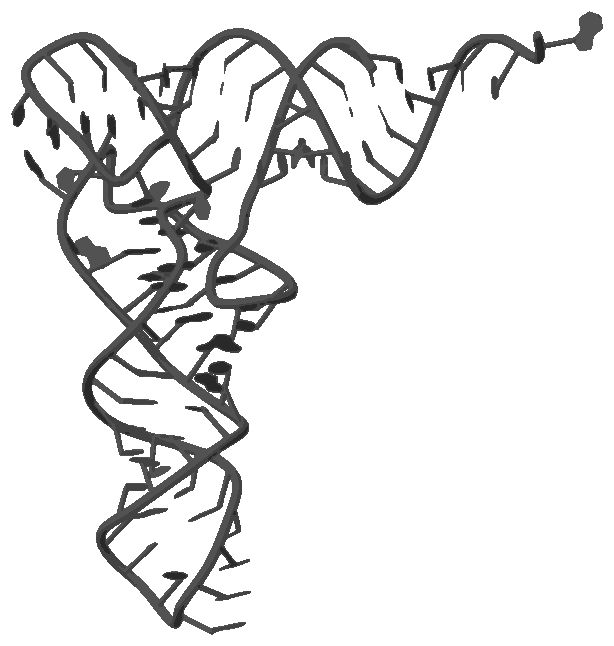
\includegraphics[width=\textwidth]{trna-3d}
    \vspace*{\fill}
\end{center}
